\chapter{Mixed Reality for Human-Robot Collaboration}   
\label{chapter:on-site}
% \chapter{On-site Member's Application}% first title of section

\begin{introduction}
    % This chapter presents the development of a comprehensive framework for implementing a Mixed Reality environment in Human-Robot Collaboration. 
    % % By allowing both on-site and remote manipulation through a communication pipeline, this system enables real-time robot manipulation and monitoring. 
    % The framework leverages advanced technologies such as Mixed-Reality, Digital Twins, and ROS, ensuring precise synchronization between physical and digital models. It discusses the tools, control methods, and User Interface enhancements designed to optimize both on-site and remote user experiences, aiming towards an intuitive, immersive collaboration.
    The primary objective of this project is to enhance remote human-robot collaboration through a framework incorporating a UR10e robotic arm and a mixed reality interface. This framework leverages real-time, bidirectional communication, allowing the mixed-reality system to function as an active, synchronized digital twin rather than a static digital replica. With an intuitive user interface, the system aims to provide remote operators with robust visualization and precise control capabilities as well as enabling seamless monitoring and manipulation of the robotic arm within the collaborative environment
\end{introduction}


\section{System Framework and Architecture}

This section details the foundational architecture enabling seamless \ac{MR} integration within the \ac{HRC} environment, connecting on-site and remote interactions. Figure~\ref{fig:project_framework} illustrates the proposed framework of the system, through a robust communication pipeline designed to enable real-time, collaborative robot manipulation.

\begin{figure}[h]
    \centering
    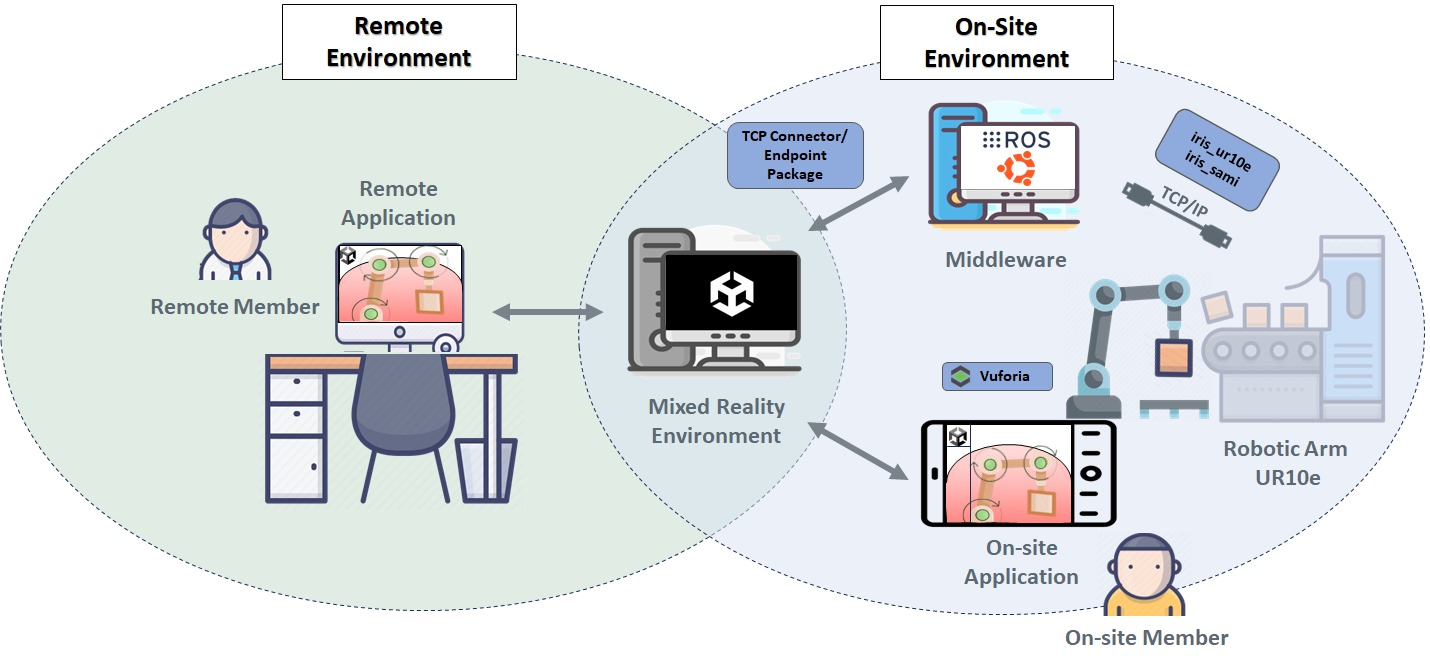
\includegraphics[width=\linewidth]{figs/framework-1.jpeg}
    \caption{Overview of the proposed \ac{MR}-based \ac{HRC} system framework integrating remote and on-site environments.}
    \label{fig:project_framework}
\end{figure}

First of all, regarding the \textbf{On-Site Environment}, the UR10e robotic arm operates as the central physical entity to be controlled. The on-site user interacts with this robotic arm through a custom \ac{MR} application developed in Unity, chosen due to its robust \ac{MR} capabilities, which facilitates the creation of immersive, interactive environments, enabling intuitive real-time robot manipulation.

After implementing the robot digital model into the simulation environment, the next step was to align it with the physical robot. Pose registration between the physical robot and its digital counterpart is executed using Vuforia's capabilities. The system employs ArUco markers for precise pose estimation, ensuring that the digital representation of the UR10e is accurately aligned with its physical counterpart. The \ac{DT} of the robot, rendered in Unity, provides a visually synchronized, real-time mirror of the robot's movements and configurations, thus facilitating enhanced interaction.

The robot is connected via Ethernet to a laptop running Ubuntu 20.04 with \ac{ROS} Noetic, which serves as the middleware layer. This setup facilitates seamless data exchange between the Unity \ac{DT} and the physical robot. The \texttt{iris\_ur10e} and \texttt{iris\_sami} \ac{ROS} packages, available on IRIS Lab's GitHub~\footnote{https://github.com/iris-ua}, provide a pre-established \ac{ROS} environment that supports critical functionalities such as trajectory planning and robotic manipulation and visualization through RViz.

To tailor these packages to the specific needs of this project, several enhancements were made. These modifications included the integration of bidirectional data flow between \ac{ROS} and Unity, enabling the Unity-based \ac{DT} to mirror the real-time movements of the physical robot. In particular, new \ac{ROS} nodes were created to subscribe to joint state data from the physical robot and publish these updates to Unity, ensuring precise synchronization between the physical and virtual environments. Additionally, new publishing mechanisms were implemented to send commands from Unity back to \ac{ROS}, allowing for full control of the robot through the \ac{MR} interface. 

This communication between the \ac{ROS} middleware and Unity’s \ac{MR} environment is established using Unity’s \ac{ROS}-\ac{TCP}-Connector and \ac{ROS}-\ac{TCP}-Endpoint packages. These packages establish communication over a \ac{TCP}/\ac{IP} protocol, ensuring real-time synchronization between the virtual and physical environments. This architecture is fundamental for maintaining the \ac{DT}'s fidelity, reflecting real-world changes in the Unity model and vice versa, as referred in the section \ref{sec:dt}.

When talking about the \textbf{Remote Environment}, this user accesses the same Unity-\ac{MR} application, allowing it to visualize and manipulate the robot from a separate location. The \ac{UI} provides real-time visualization of the robot’s state and its workspace, enabling remote collaboration. The synchronization between the remote and on-site environments is facilitated through Unity’s \ac{MR} capabilities, which, in conjunction with the \ac{ROS}-based control, enables the remote user to execute commands and receive real-time feedback.

The Middleware layer, acting as the system’s backbone, ensures the continuous synchronization of data between the physical robot and its \ac{DT}. It manages the real-time feedback loop, maintaining bidirectional data flow between the virtual robot in Unity and the physical robot in the on-site environment. This configuration guarantees that any actions performed by either the on-site or remote user are consistently reflected in both the physical and digital realms, preserving operational coherence and maximizing collaborative efficiency.

This framework aims to provide an immersive and responsive \ac{MR} environment, bridging the gap between physical and digital spaces. The system enables real-time robot manipulation and monitoring from both on-site and remote locations, making it a versatile platform that could be used for collaborative tasks in advanced industrial applications. Seamless integration between \ac{MR} and \ac{DT} within \ac{HRC} technologies significantly enhances user interaction, safety, and productivity, while offering an intuitive interface for remote and on-site collaboration.


\section{Robot Manipulation Within Mixed Reality Environment}

Building on this comprehensive framework, the Unity-based \ac{MR} environment is designed to implement and control the \ac{DT} representation of the UR10e robotic arm. Initially, basic robot manipulation was achieved through the Unity Robotics Hub's \ac{URDF} Importer, enabling joint-specific adjustments via keyboard controls. However, to enhance user interaction and provide a more intuitive experience, new control methods were subsequently developed within the application, aimed at optimizing the user’s ability to monitor and interact with the robotic arm in real time. This section outlines these control methods in detail, describing their specific functions and contributions to the \ac{HRC} experience.

In order to properly develop new ways of controlling the \ac{DT} version of the robot, it was necessary to understand the core C\# script which contained all the necessary functions to control the robot's joints within Unity, named \texttt{Controller.cs}. After further analysis, control methods were implemented to facilitate the manipulation of the digital robot model through a \ac{HHD} interface. This interface includes a menu displaying each joint, enabling users to adjust the robot’s position directly. Once the digital model is set to the desired position—either via the \ac{HHD} or keyboard controls—the user can publish this position to the \ac{ROS} middleware, which moves the physical robot accordingly. Additionally, another method was created for situations where the on-site counterpart manipulates the physical robot directly. In these cases, the \ac{DT} mirrors the real robot’s movements, maintaining synchronized operation between the physical and virtual environments.

These methods are explained in detail below.


\subsection{UI Control Panel and Joint Manipulation}
\label{subsection:ui-control-method}
% \textbf{UI Control Method}:
This method is designed to provide users with an intuitive, user-friendly interface for manipulating the \ac{DT} of the UR10e robot. 

Figure \ref{f:ui-control} illustrates the \ac{UI} developed in Unity, highlighting its primary control panel on the left (1), which includes a detailed joint selection menu, directional arrows, and a reference image of the robot with joint labels (2 and 3). This panel is central to controlling the digital model of the robot, while other \ac{UI} features shown in the figure will be explained in subsequent sections.

\begin{figure}[h]
    \centering
    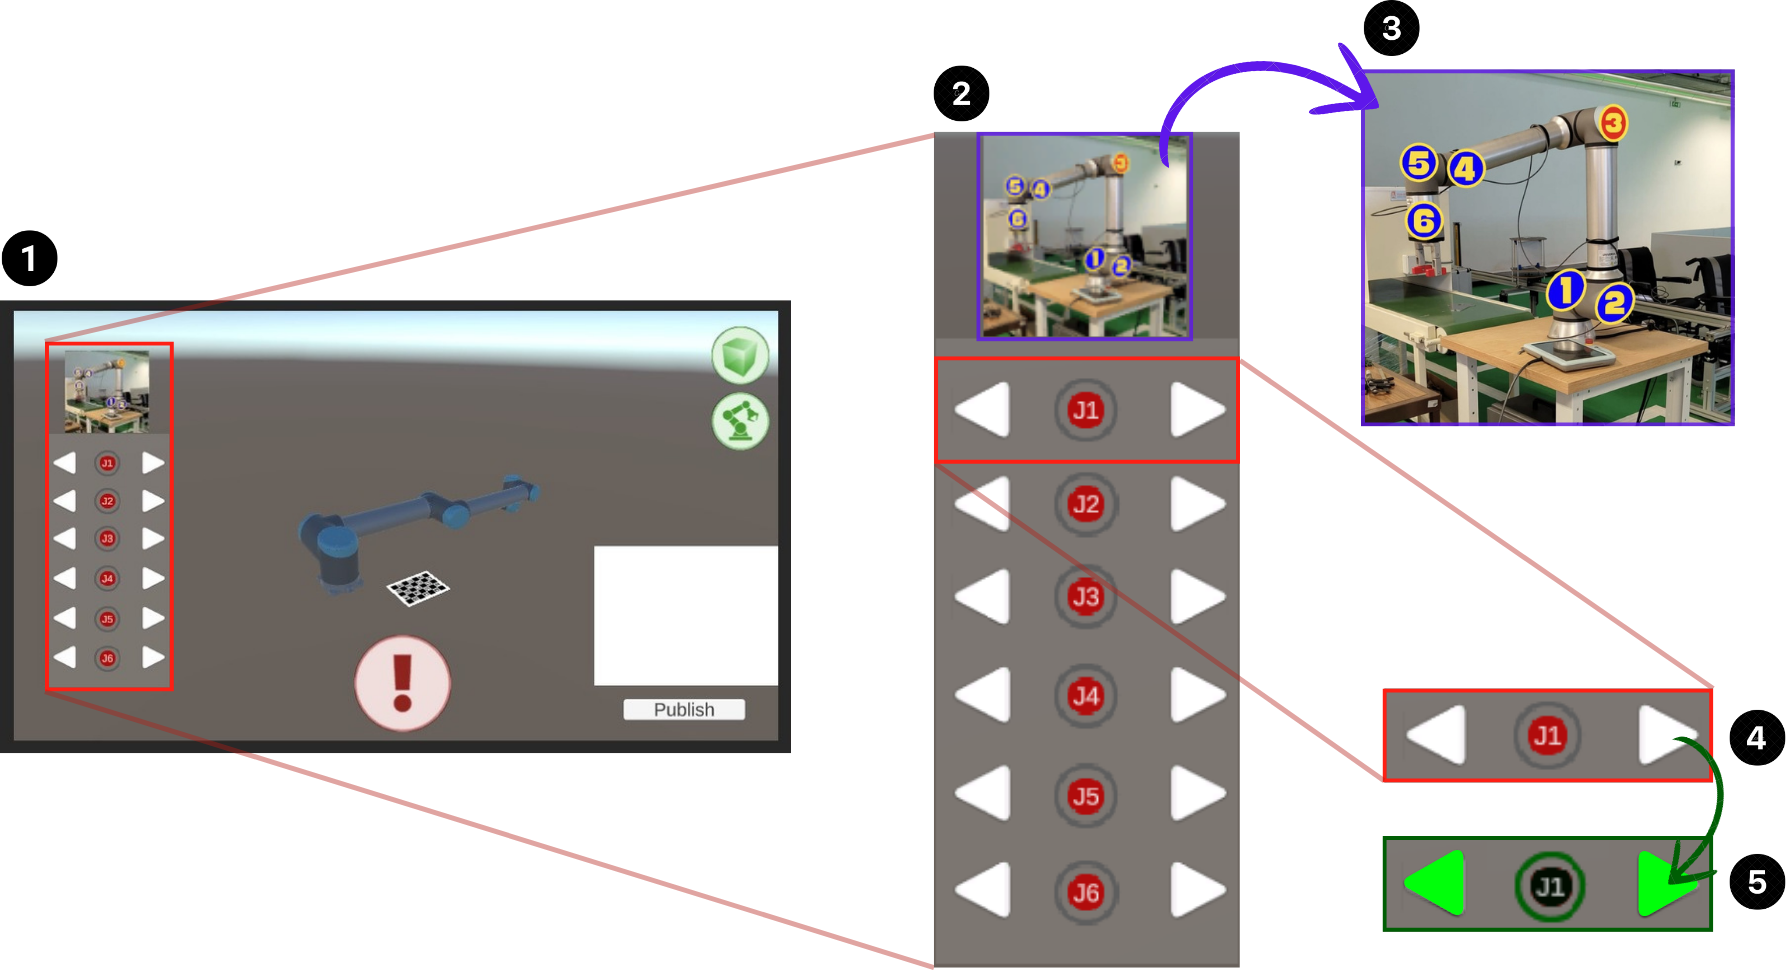
\includegraphics[width=\textwidth]{figs/interface-numerada-2.png}
    \caption{\ac{MR} \ac{UI} in Unity simulation environment (1). The control panel (2) enables the manipulation of the UR10e robot digital model. Users can manipulate each joint individually, with active joints displayed in green to indicate selection (5). The reference image of the robot (3), labeled with joint numbers (J1 to J6), aids in joint identification from base to end-effector. Directional arrows for each joint (2,4,5) facilitate movement control in positive or negative directions, offering intuitive joint-level manipulation within the simulation.}
    \label{f:ui-control}
\end{figure}


\textbf{Interface Structure and Joint Manipulation}:
\begin{itemize}
    \item \textbf{Joint Selection:} Each joint has a central button labeled with its identifier (e.g., J1, J2). To activate a joint, the user clicks the corresponding button, which changes color from red to green, signaling that the joint is selected for movement (4 and 5). This selection process helps avoid confusion and accidental manipulation of multiple joints.

    \item \textbf{Movement Control:} Once a joint is selected, the user can manipulate its position by clicking the directional arrows on either side of the central button. Pressing the right arrow rotates the joint in the positive direction, while the left arrow rotates it in the negative direction. This control mirrors the real-time responsiveness typically provided by keyboard arrows, ensuring an intuitive experience.

    \item \textbf{Continuous Movement:} The selected joint will continue moving in the chosen direction as long as both the central control button and the directional arrow remain selected. To stop the movement, the user can deselect either the joint by clicking on the central button or its rotational arrow, reverting these elements to its default color.

    \item \textbf{Single Joint Activation: }Only one joint can be active for rotation at any time. If multiple joints are selected (i.e., their buttons are green), the system prevents movement in any direction until only one joint is selected.

    % \item \textbf{Directional Exclusivity}: When a rotation direction is chosen (e.g., pressing the right arrow), the opposite direction is temporarily disabled, as shown in Figures 4 and 5. This feature prevents conflicting commands, reinforcing safe and logical control of the robot.
\end{itemize}

\textbf{Additional Design Considerations: }
\begin{itemize}
    \item \textbf{Visual Reference for Joint Positioning:} The overlay image at the top of the joint control panel serves as a quick-reference guide for users to confirm joint positions relative to the physical robot. This visual aid is useful in remote collaboration or complex tasks where clear identification of each joint’s location is essential.

    % \item \textbf{UI Responsiveness and Feedback:} To ensure a smooth interaction, the interface provides visual feedback for each action (e.g., button color changes) and restricts movement based on user inputs, making the control process both transparent and manageable.
\end{itemize}

This structured approach to joint manipulation tries to promote safe, precise, and efficient interaction with the robot, supporting the usability goals of the \ac{MR} application. By minimizing the likelihood of accidental commands and providing continuous, clear visual feedback, the interface helps maintain control clarity and operational awareness throughout the interaction.
% The design is especially advantageous in collaborative environments, where multiple participants may need to observe and understand the robot’s operations in real time.


\subsection{Unity to Robot}
% \textbf{Unity-ROS Control:} 
Similarly to the previous described method, this one also enables the digital robot model to be controled from the \ac{MR} environment. However, when needed, it sends the newly defined digital robot position into the Middleware environment, updating the real UR10e robot status. In order to change the \ac{DT}, the user has can also do it by pressing the right/left arrow keyboard keys to select the following/previous joint as well as the up/down keys to rotate the selected joint in the positive/negative direction, respectively.
        
After moving the digital model to the desired position, by pressing the "Publish" button within the \ac{UI}, as shown in Figure \ref{fig:publish_UI_button}, the robot's joints coordinates are published to the \ac{ROS} middleware, using the \ac{ROS}-\ac{TCP}-Connector/Endpoint packages.


\begin{figure}[htpb]
    \centering
    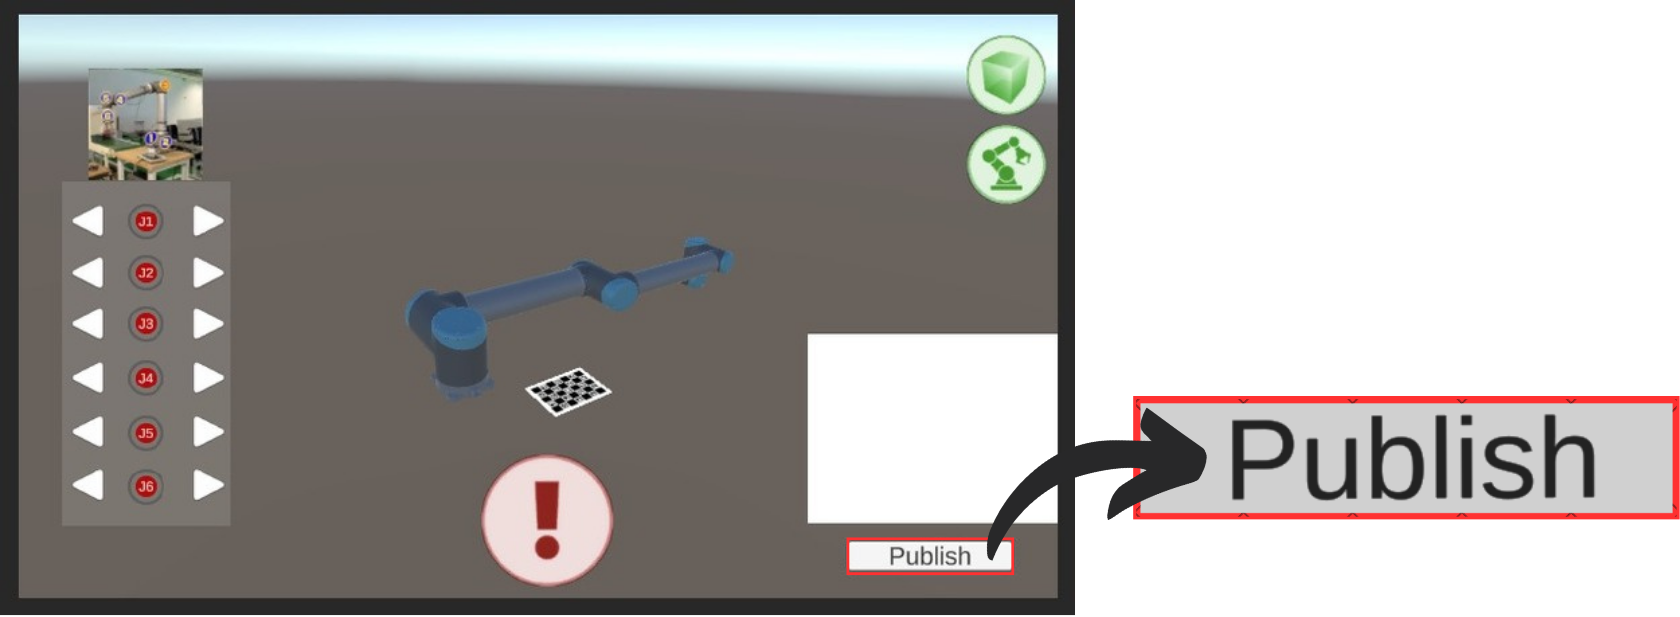
\includegraphics[width=0.8\linewidth]{figs/publish-button.png}
    \caption{Publish button that sends Unity's \ac{DT} robot joint states into ROS the environment}
    \label{fig:publish_UI_button}
\end{figure}

To avoid conflicts with the \ac{ROS} node responsible for controlling the real robot's joints, which are being constantly published to the standard \texttt{/joint\_states} topic, a separate \ac{ROS} topic \texttt{(/unity\_joint\_states)} was created to handle the joint data coming from Unity. This ensures that data from Unity does not interfere with the real robot’s ongoing operations. When the "Publish" button is pressed, the Unity-defined joint states are sent to this new topic, and only when necessary are they relayed to the real robot for movement execution. Algorithm \ref{alg:unity_input} represents a pseudo-code snippet that explains how to update the \ac{DT} in Unity and send the new desired robot position to the \ac{ROS} middleware.

\begin{algorithm}
    \caption{Unity Input for Joint Selection and Movement}\label{alg:unity_input}
    \begin{algorithmic}[1]
        \State \textbf{Step 1: User Input for Joint Selection and Movement in Unity}
        \While{Unity Simulation is running AND Unity-ROS Control is enabled}
            \If{RightArrowKeyPressed}
                \State Select next joint
            \ElsIf{LeftArrowKeyPressed}
                \State Select previous joint
            \EndIf
            \If{UpArrowKeyPressed}
                \State Rotate selected joint in positive direction
            \ElsIf{DownArrowKeyPressed}
                \State Rotate selected joint in negative direction
            \EndIf
            \If{PublishButtonPressed}
                \State joint\_states = GetCurrentJointStates()
                \State PublishToROSTopic(/unity\_joint\_states, /joint\_states)
            \EndIf
        \EndWhile
    \end{algorithmic}
\end{algorithm}


In order to handle this communication process, two new \ac{ROS} nodes were created, \texttt{joint\_state\_listener} and \texttt{move\_unity}. The \texttt{unity\_joint\_subscriber.py} script was developed within the \texttt{iris\_ur10e} package, initializing the node that subscribes to the \texttt{/unity\_joint\_states} topic, which receives a JointState message type. It then starts the publisher for the \texttt{/move\_joint\_unity} topic, converting this data into a Float64MultiArray format which will be further received by the second node. This second node called \texttt{move\_unity}, created within the \texttt{iris\_sami} package, subscribes to the \texttt{/move\_joint\_unity} topic, listening to new joint position values, moving the robotic arm to this desired position. This real-time update can be visualized either on the simulation environment, through Rviz, or by utilizing the real UR10e robot. Another pseudo-code algorithm explanation regarding how both \ac{ROS} nodes work, is presented in \ref{alg:combined_ros_node}.

% Part 2: ROS Node for Receiving Unity Joint States

\begin{algorithm}
    \caption{Combined ROS Node for Receiving Unity Joint States and Moving the Robot}\label{alg:combined_ros_node}
    \begin{algorithmic}[1]
        \State \textbf{Step 2 and 3: Combined ROS Node for Receiving Unity Joint States and Moving the Robot}
        
        \State Initialize ROS Node: joint\_state\_listener
        \State Subscribe to Topic: '/unity\_joint\_states'
        
        \While{Receiving JointState message from Unity}
            \State float\_array\_data = ConvertToFloat64MultiArray(joint\_states)
            \State PublishToROSTopic('move\_joint\_unity', float\_array\_data)
        \EndWhile
        
        \State \textbf{Precondition:} The \texttt{joint\_state\_listener} node must be running and publishing to the \texttt{'/move\_joint\_unity'} topic.
        \State Initialize ROS Node: test\_arm\_movement
        \State Subscribe to Topic: '/move\_joint\_unity'
        
        \While{Receiving Float64MultiArray message from \texttt{move\_joint\_unity}}
            \State MoveRobotArmTo(joint\_positions)
            \If{ConnectedToRealRobot}
                \State MoveRealRobot()
            \Else
                \State VisualizeInRviz()
            \EndIf
        \EndWhile
    \end{algorithmic}
\end{algorithm}


    
\subsection{Robot to Unity}

Opposite to the above described method which controlls the \ac{DT} and then updates the robot position, in this control method, the on-site user moves the robot and the remote counterpart visualizes this update instantly within the \ac{MR} environment.

In order to properly achieve this communication and data transfer, the \texttt{JointStateSubscriber.cs} script was created in Unity. It subscribes to the \texttt{/joint\_states} topic, and stores the information regarding the joint positions in a dictionary structure that is updated in real time into a specific \texttt{.json} file within the \ac{MR} environment. This file is constantly being read by the \texttt{Controller.cs} script whenever this control method is enabled, updating the \ac{DT} robot model accordingly.

By maintaining this synchronization between the real robot and the virtual environment, the Unity scene accurately reflects the robot's live state, ensuring a consistent \ac{DT} representation through the bidirectional communication established between the \ac{MR} environment and the \ac{ROS} middleware. Below, algorithm \ref{alg:ros_unity_control} explains how this \ac{ROS}-Unity control method works.


\begin{algorithm}
    \caption{ROS-Unity Control via Joint States Subscription}\label{alg:ros_unity_control}
    \begin{algorithmic}[1]
        \State \textbf{Step 1: Subscribe to ROS \texttt{/joint\_states} topic}
        \State Attach the Unity Script to the Digital Robot Model Asset: \texttt{JointStateSubscriber.cs}
        \State Upon Initialization, it subscribes to topic: \texttt{/joint\_states}

        \While{Receiving JointState message from \ac{ROS}}
            \State Extract joint names and positions from the message and store them in a dictionary data structure
            % \State Store them in a dictionary structure
            \State Save the dictionary data to the \texttt{jointStateSubscriber.json}
        \EndWhile

        \State \textbf{Step 2: Update Unity \ac{DT} Robot Model}
        \While{Simulation is Running}
            \State Read the \texttt{jointStateSubscriber.json}
            \State Update the Unity \ac{DT} robot model using the joint positions from the dictionary structure
        \EndWhile

        \State \textbf{Step 3: Synchronize Real Robot with \ac{DT} Robot}
        \State The Unity \ac{DT} robot model moves according to the real robot’s joint positions, ensuring a consistent bidirectional \ac{DT} representation.
    \end{algorithmic}
\end{algorithm}

Figure~\ref{fig:robot-unity} illustrates this real-time synchronization between the UR10e robot and its \ac{DT} within the \ac{MR} environment. As the on-site user manipulates the physical robot, its digital counterpart updates instantly within Unity, providing the remote user with a synchronized visual representation of the robot’s movements.

\begin{figure}[h]
    \centering
    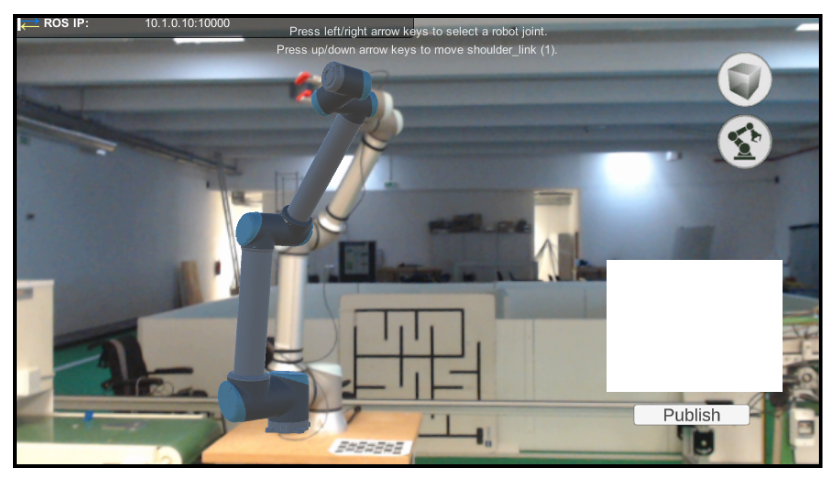
\includegraphics[width=\linewidth]{figs/super-imposed-robot.png}
    \caption{Real-time synchronization of the UR10e robot’s \ac{DT} in Unity environment, showing an accurately overlay of the robot. This synchronization enables remote users to monitor the robot's state within the \ac{MR} environment, reflecting live updates via bidirectional \ac{ROS}-Unity communication}
    \label{fig:robot-unity}
\end{figure}


\section{Mixed-Reality Features}
\label{section:on-site-features}
% \input{chapters/on-site/on-site-features} commented this part because text is below - choose whether to use this or the text below
After having implemented the \ac{DT}-Robot bidirectional communication between the on-site and remote members, the next step consisted on developing features that could enhance both users' experience when interacting with the collaboration environment. These features were designed to improve user safety, facilitate robot manipulation, and provide an intuitive interface. The following sections detail these key features development and implementation.

% Regarding the on-site member's collaboration experience, as explained in the state of art review, by implementing different sensorial cues, such as visual and audio, it will enhance the user experience into a more intuitive and immersive way.

\subsection{Virtual Safety Zones and Sensorial Cues}
\label{subsection:virtual-safety-zones} 
% \input{chapters/on-site/subsections/virtual-safety-zones} commented this part because text is below - choose whether to use this or the text below

As explained in section \ref{sec:hrc-in-industry}, introducing different sensorial cues enhances on-site users' experience into a more intuitive and immersive experience. Therefore, visualizing the working zone of the robot is a critical feature designed to enhance safety when interacting with the robot. Figure \ref{fig:safety-zones} displays the developed safety-zones that aim to increase awareness around the robot's working space. Alongside these two safety zones' development, other features that address specific safety and user's concerns are explained below:  

\begin{figure}[h]
    \centering
    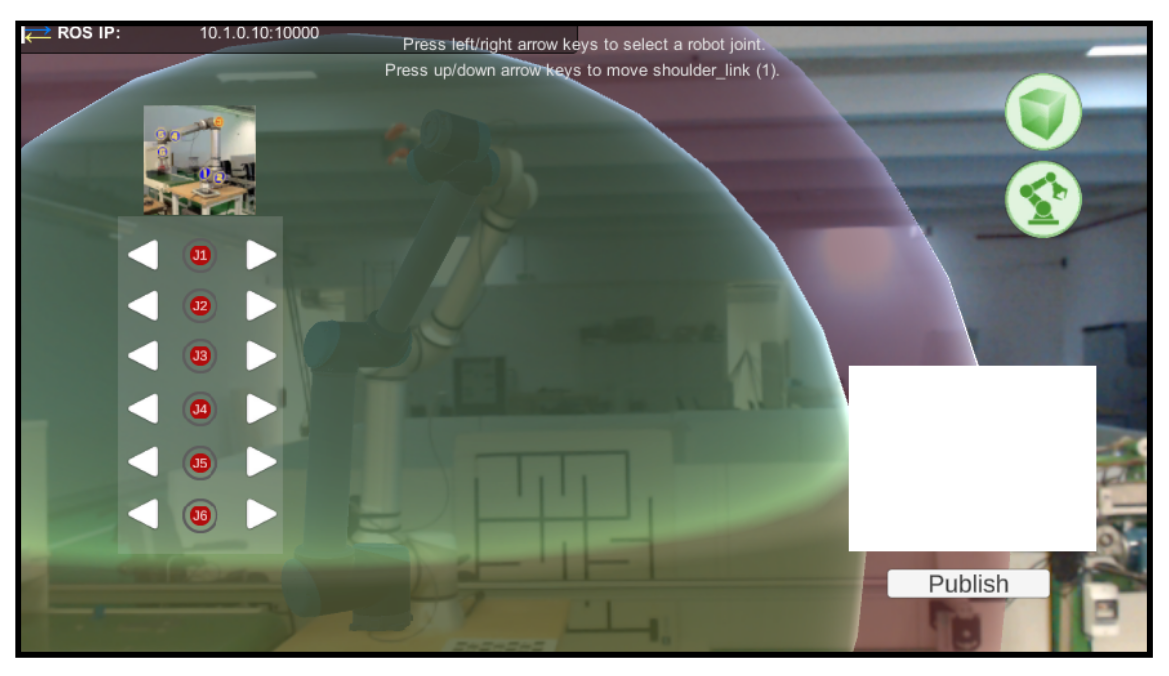
\includegraphics[width=\linewidth]{figs/safet-zones.png}
    \caption{\ac{MR} application \ac{UI}, with safety-zones aumenting the robot's working area in order to address user's safety}
    \label{fig:safety-zones}
\end{figure}

\begin{itemize}
\item \textbf{Outer Safety Zone:} Initially, only this safety zone was created. The purpose of creating it was to provide an 
early warning to users as they approach the hazardous area near the robot. This approach consisted on changing its color as a visual alert. 
However, this method proved ineffective because, once inside it, users could not perceive the color change, rendering the warning system inadequate.

\item \textbf{Inner Safety Zone:} To overcome this outer zone limitation, an additional Inner-Safety Zone was developed. This design ensures a two-step safety mechanism that properly alerts users when they are in close proximity to the robot.

\item \textbf{Sensorial Cues:  }
\textbf{Visual}: Upon entering the Outer-Safety Zone, the color of the Inner sphere changes to red, reverting to its default color if the user exits this critical area. This visual cue alerts the user to increased proximity to a high-risk zone. Additionally, a blinking warning appears at the bottom center of the interface, switching between both circular danger signs shown in Figure \ref{fig:blinking-sign}. This flashing indicator amplifies the alert, reinforcing the awareness of approaching the operational robot area, remaining active as long as the user is within this Outer-Safety Zone.


\textbf{Auditory}: Entering the Inner-Safety Zone triggers an audio alarm signifying that the user has breached into the robot working area, enhancing the effectiveness of the safety mechanism.

\begin{figure}[h]
    \centering
    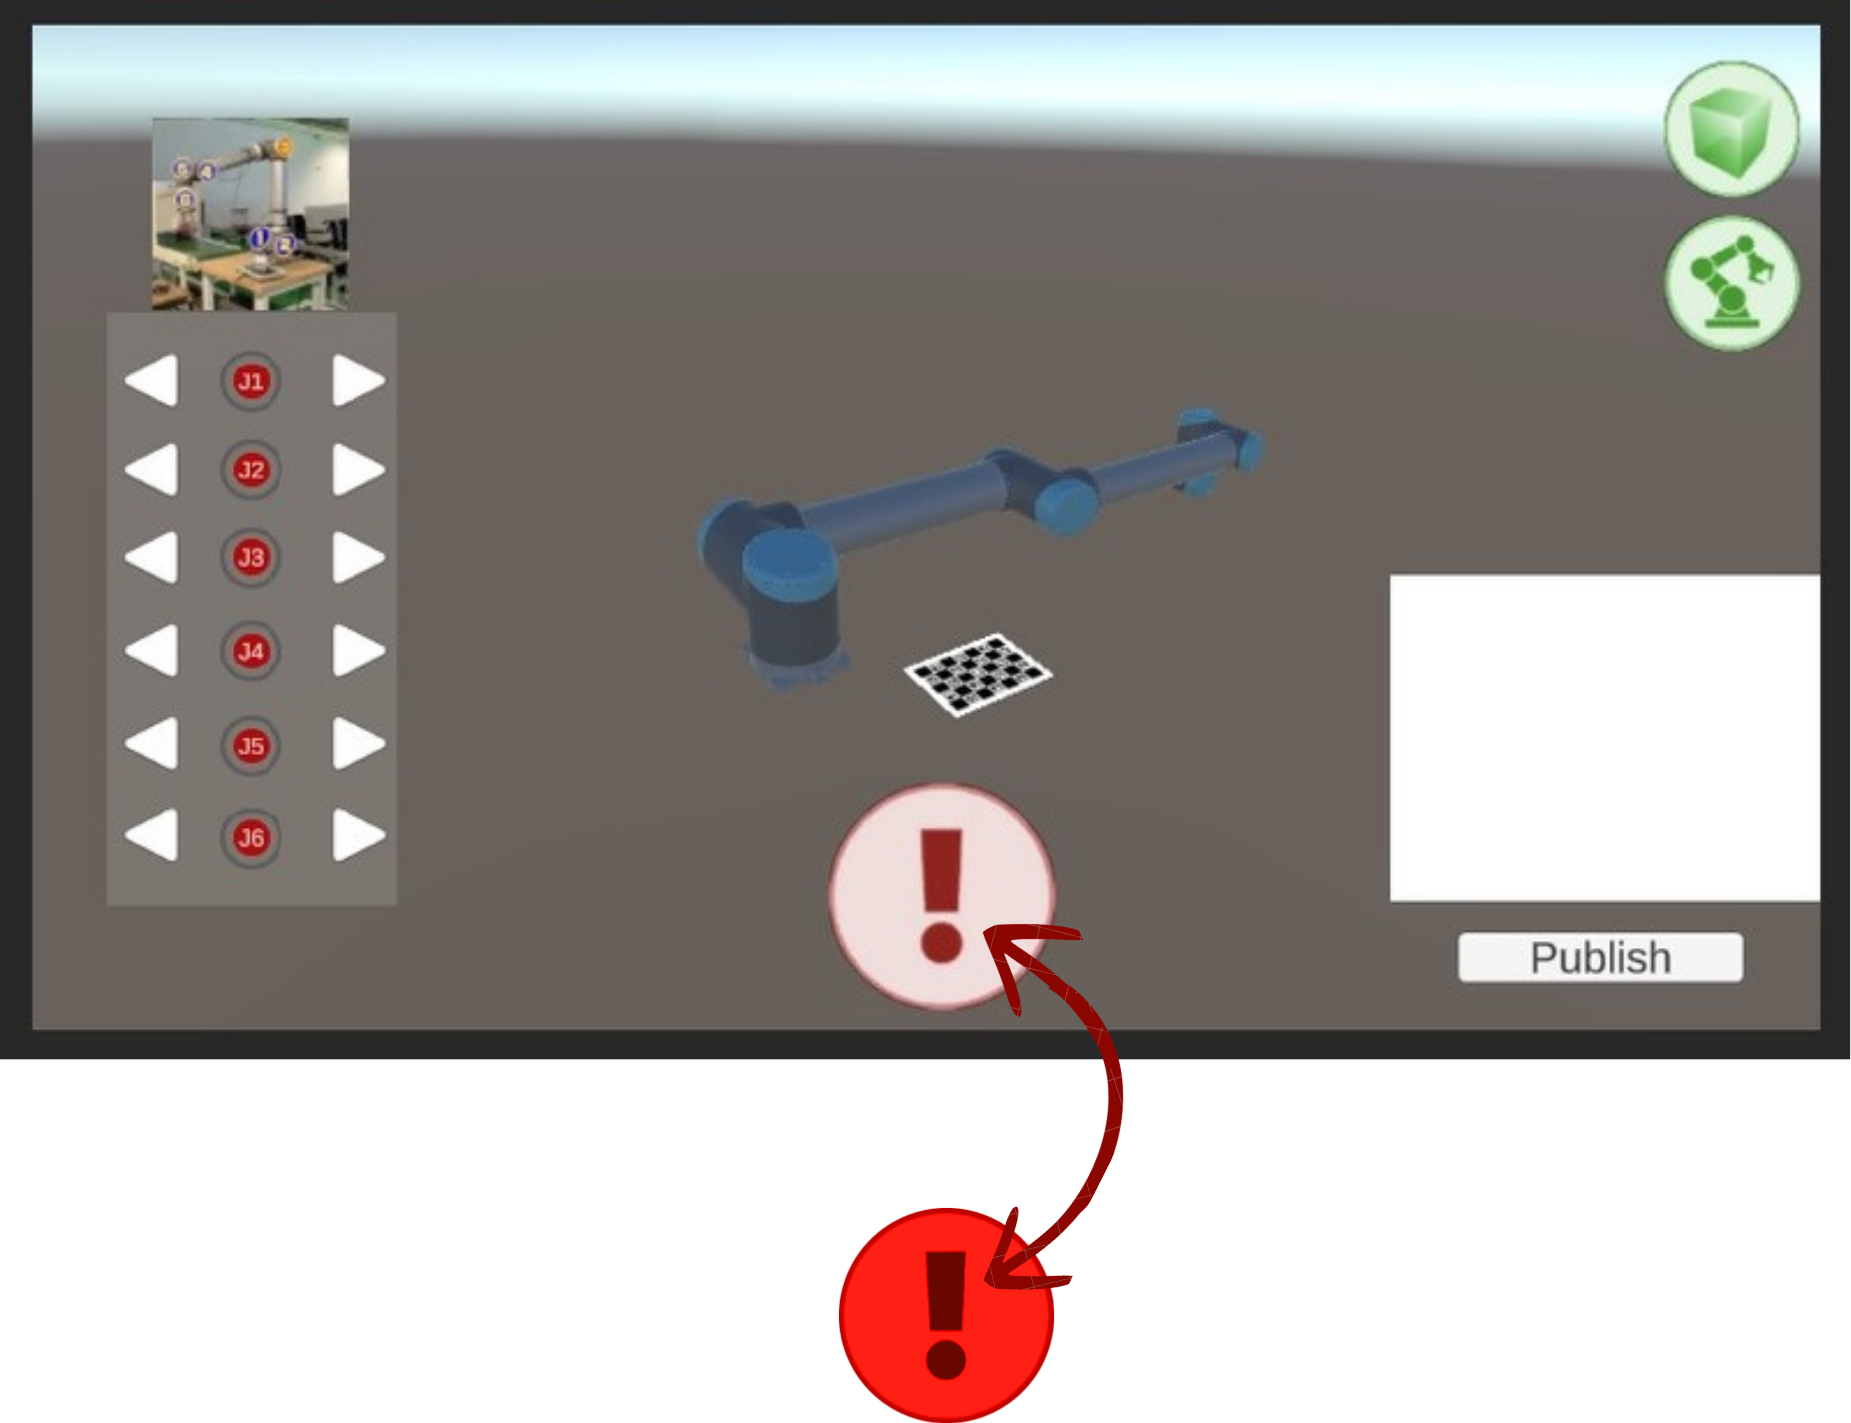
\includegraphics[width=0.7\linewidth]{figs/sign-alert.png}
    \caption{Warning blinking sign displayed in the bottom part of the \ac{UI} to alert the on-site user of proximity to the Robot}
    \label{fig:blinking-sign}
\end{figure}

\item \textbf{Breach Protocol:} Besides the above described sensorial cues whose goal consists on improving user's awareness, another feature was implemented to ensure user's safety when interacting with the robot. If the on-site counterpart enters the Outer-Safety Zone while the robot is in motion, the robot automatically stops. This immediate halt ensures that potential accidents or injuries are avoided by preventing any interaction with the robot when a user is within this designated dangerous area.
\end{itemize}
    
% this interface section - the feature of controlling it using the UI must be put in the UI COntrol method above
%  the remaining part should be in this part - explaining the rest of the UI features
\subsection{Flexible Interface Options for User Customization}

Beyond the joint control panel displayed on Figure \ref{f:ui-control}, several additional features were integrated into the \ac{MR} application aimed at enhancing user flexibility and clarity. Positioned in the upper right corner of the \ac{UI}, two green toggle buttons provide control over distinct interface functionalities.

By utilizing these two toggle buttons, users can enable/disable the visibility of both safety zones and the robot joint control panel for an optimized workspace view. Figure \ \ref{fig:all-features-button} demonstrates this \ac{MR} interface flexibility. In image 1, both safety zones and control panels are active. By selecting the upper-right button, the user can deactivate safety zones, turning this toggle button into gray and thus, removing visual cues and safety-zones related features (2). The lower button, pressed in image 3, toggles the robot joint control panel on and off, as illustrated in image 4. This toggle also behaves in the same way of the above one, turning into gray upon deactivation. Image 5 represents the deactivation of both features, achieving an unobstructed view. These customization options allow users to adjust the interface according to task requirements, balancing between safety feedback and workspace clarity.

\begin{figure}[h]
    \centering
    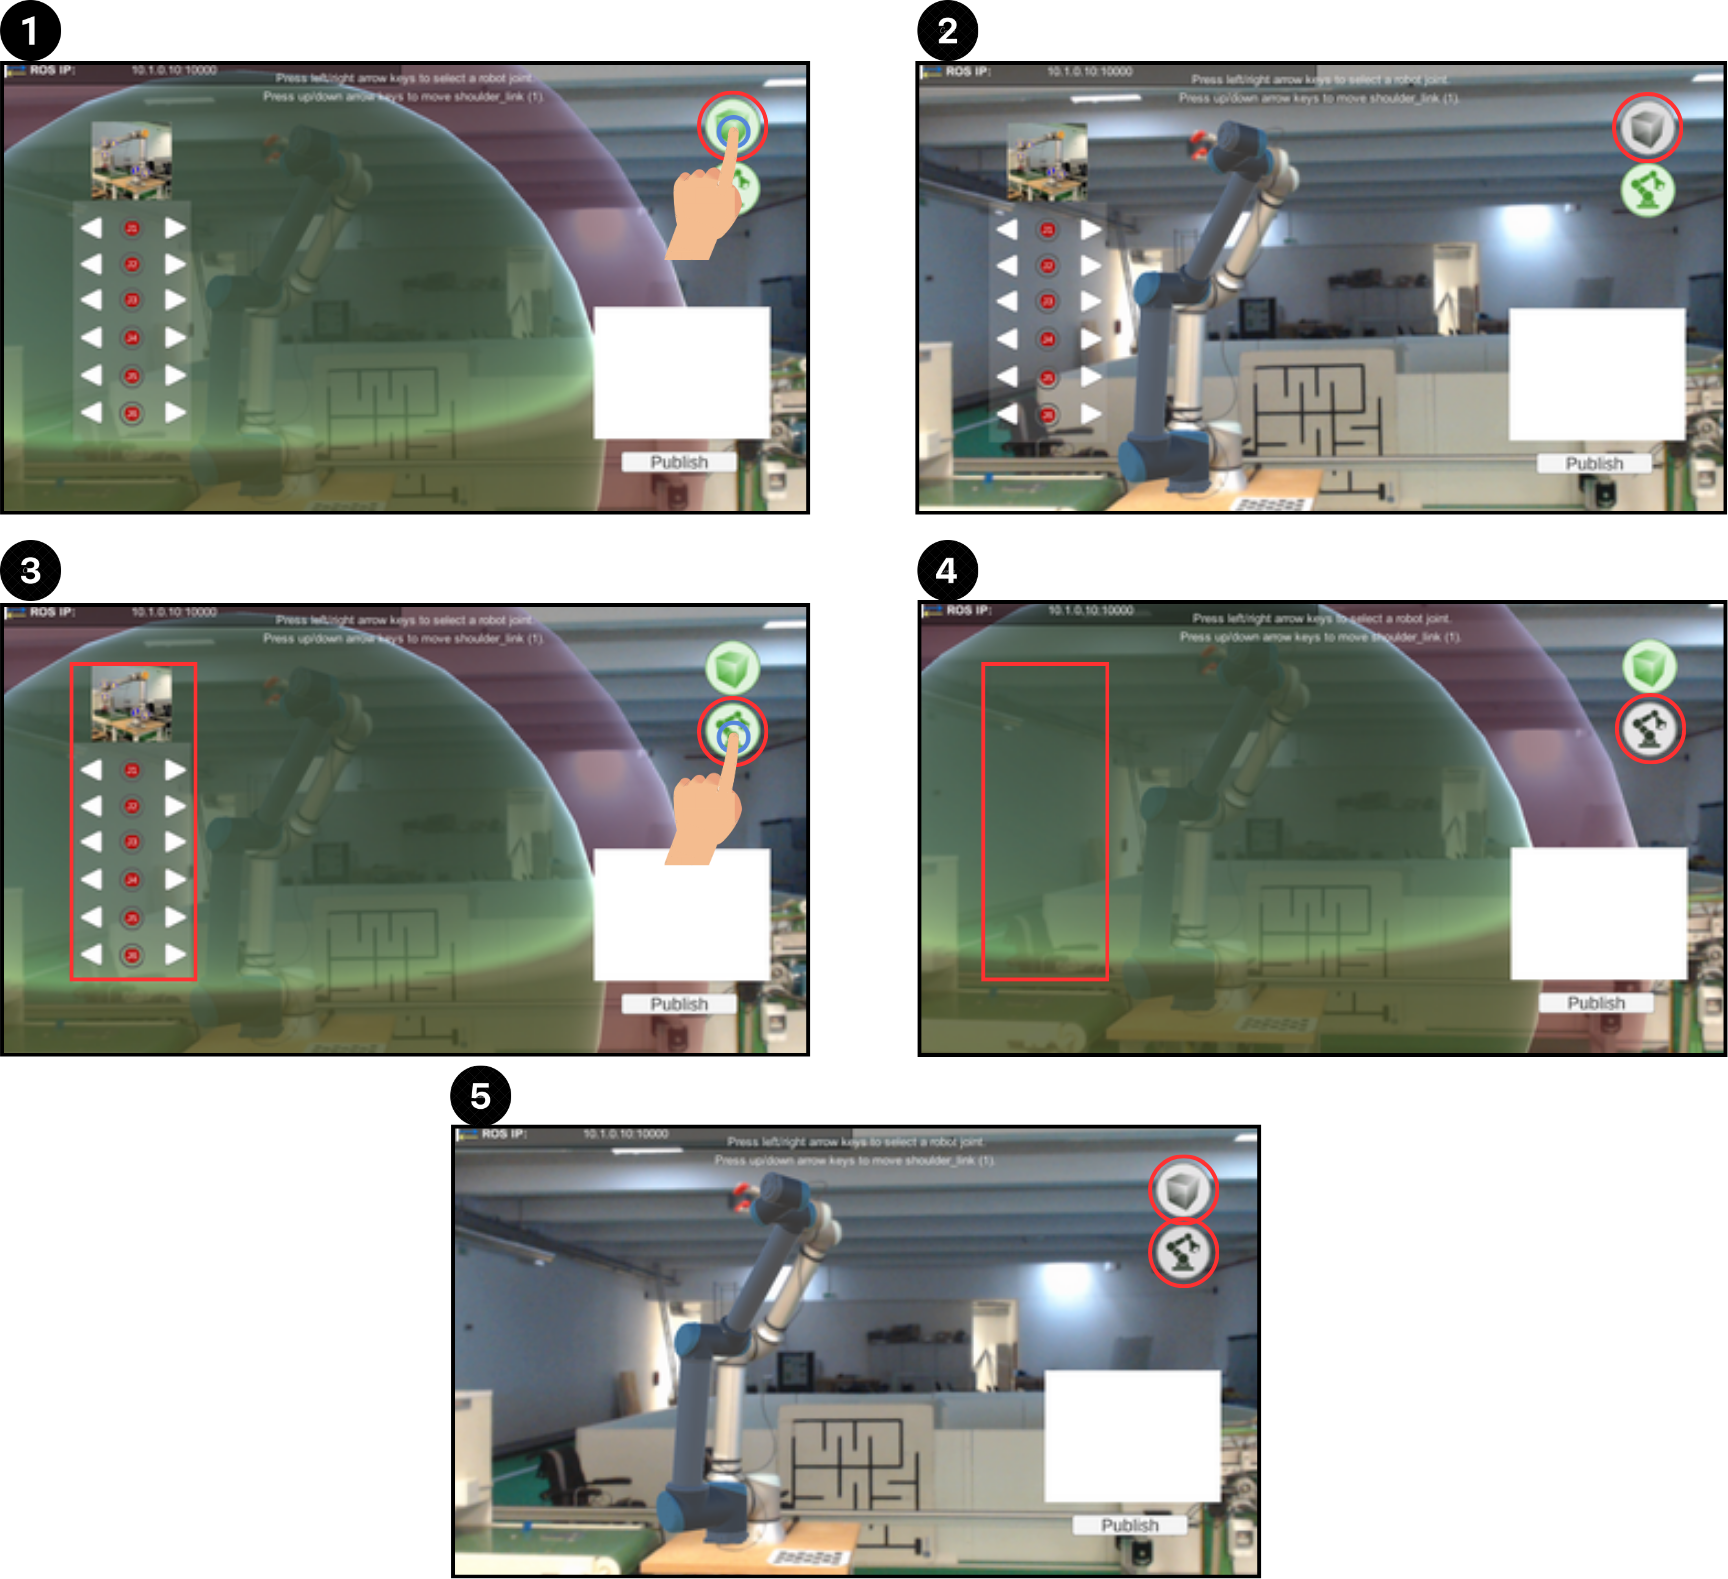
\includegraphics[width=\linewidth]{figs/all-features.png}
    \caption{\ac{UI} demonstrating the activation and deactivation of the safety zones and robot joint control panel within the \ac{MR} environment. In (1), the workspace is displayed with the safety zones active. By pressing the top-right button in (2), these zones are deactivated, providing a clearer view. In (3), pressing the button below the top-right icon deactivates the joint control panel, as seen in (4). In (5), with both buttons deactivated, the workspace is entirely unobstructed, offering maximum clarity for the user}
    \label{fig:all-features-button}
\end{figure}



\subsection{Enhanced Remote Visualization Through Camera Feed Transmission}

To improve situational awareness for remote users, an additional camera was integrated, providing real-time visual context directly from the robot’s perspective and reducing on-site operator's responsibility for managing environmental views.

The Orbbec Astra 3D camera~\footnote{\url{https://www.orbbec.com/products/structured-light-camera/astra-series/} Acessed:2024-10-22}, shown in Figure \ref{fig:astra-camera}, was chosen for its high-resolution video output and compatibility with the \ac{ROS} framework. This camera was mounted directly onto the robot, offering an immersive view that aligns with the robot’s operational perspective. Integration into the \ac{ROS} environment was facilitated through the Astra camera’s dedicated GitHub repository~\footnote{\url{https://github.com/orbbec/ros\_astra\_camera} Accessed: 2024-10-04}, which provided essential drivers and nodes for \ac{ROS} compatibility.

\begin{figure}[h]
    \centering
    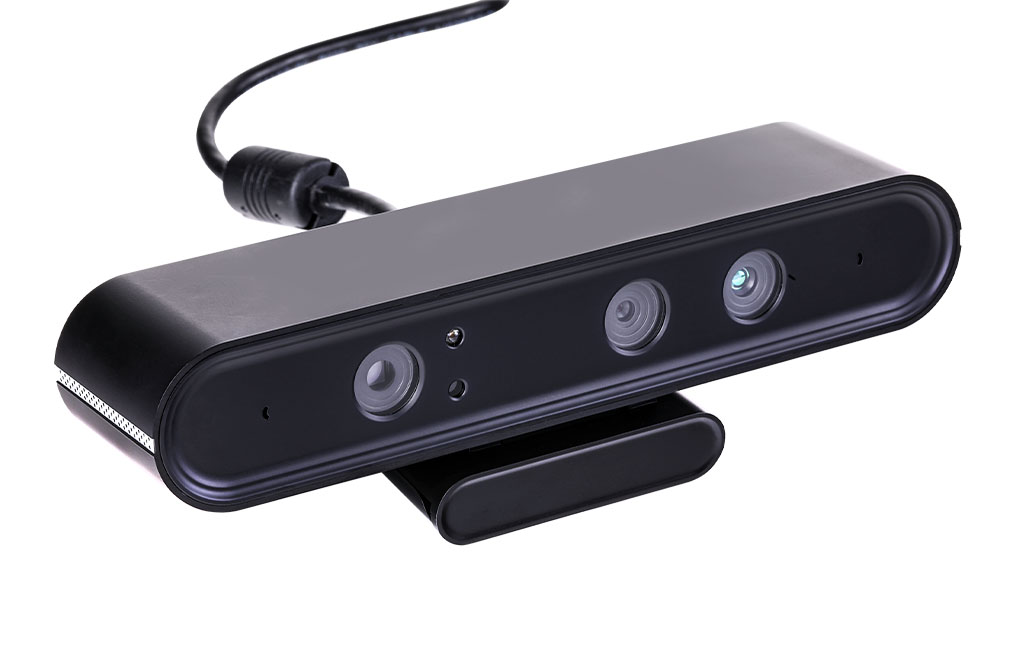
\includegraphics[width=0.5\linewidth]{figs/AstraSeries_3.jpg}
    \caption{Orbbec Astra 3D camera mounted on the UR10e robotic arm, providing a real-time visual feed of the robot's environment to support remote user awareness}
    \label{fig:astra-camera}
\end{figure}

The live feed from the Astra camera was managed via the \texttt{astra\_camera\_node} from the \texttt{astra\_camera} package, enabling continuous data capture and real-time display in RViz for preliminary verification. This configuration ensured proper camera functionality within the \ac{ROS} environment and accurate data capture. 

However, when transmitting the uncompressed image data to the Unity \ac{MR} application, bandwidth and latency challenges arose, potentially impacting real-time collaboration. To address this, the \ac{ROS} \texttt{image\_transport} package was implemented, which converted the raw video stream into a compressed format, reducing data size while preserving essential image quality. By compressing the image data, the system achieved more efficient and stable real-time transmission to Unity, providing continuous visual feedback with minimal latency. The following command facilitated the data compression:

\begin{verbatim} 
    rosrun image_transport republish raw in:=/camera/color/image_raw 
    out:=/camera/image_repub 
\end{verbatim}

Afterwards, this compressed camera feed had to be integrated into Unity. To do this, the \texttt{CameraFeedReceiver.cs} script was developed, responsible for receiving and rendering the feed into the \ac{UI} panel. This setup allowed the remote user to view the robot’s perspective in real time, independent of the on-site operator’s actions. This dual-view capability offers the remote user a comprehensive visual overview by combining the on-site provided view with the camera feed directly from the robot’s perspective, potentially enhancing spatial awareness and operational context.

Figure \ref{fig:camera-feed} demonstrates the live feed display in Unity, showcasing how the system allows remote users to monitor the robot’s surroundings and adjust their commands accordingly. This feature may support more informed decision-making in future implementations of remote \ac{MR} systems for \ac{HRC}.

\begin{figure}[h]
    \centering
    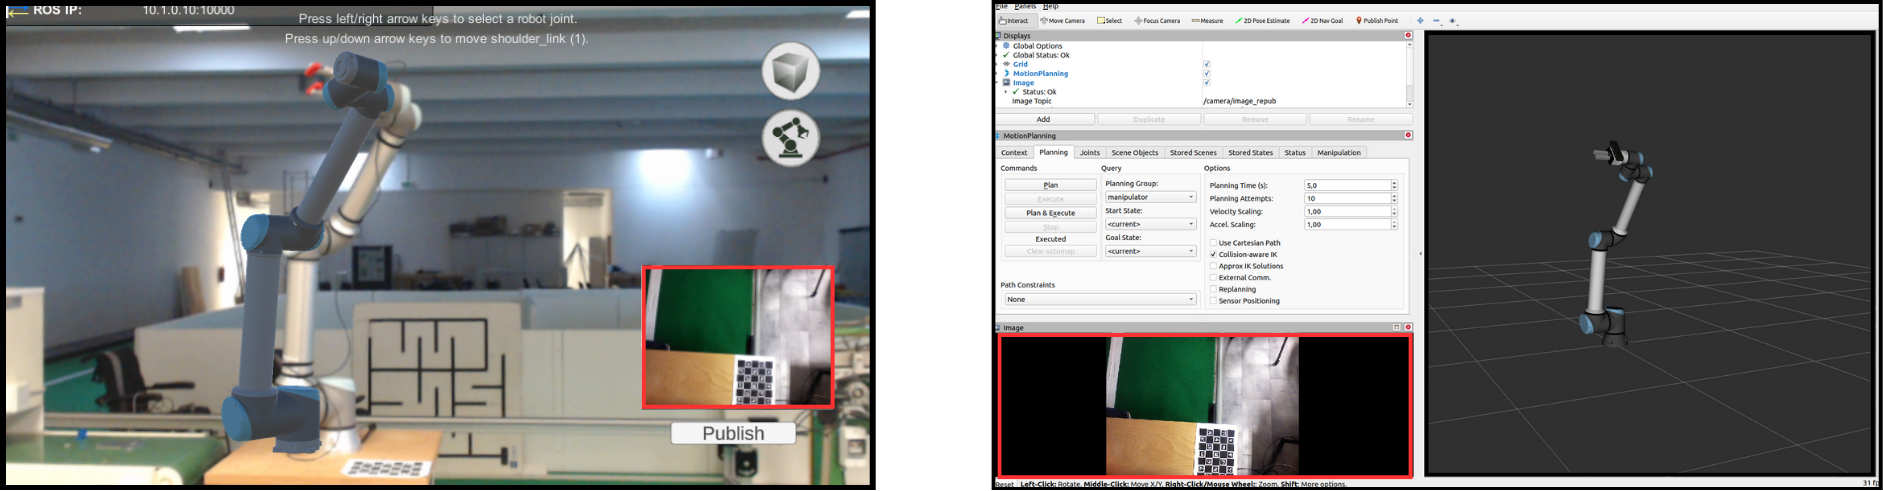
\includegraphics[width=\linewidth]{figs/camera-feed-transmission-3.png}
    \caption{Real-time camera feed integration from the robot’s perspective within the \ac{MR} environment. On the left image, Unity displays the \ac{MR} interface seen by the remote user, with emphasis on the live feed coming from the camera mounted on the robot, aiming to enhance situational awareness. The right picture shows the RViz simulation where the camera feed is captured through the \ac{ROS} Middleware setup. This live camera transmission between on-site and remote users has to be compressed, ensuring the proper quality and minimal latency between environments, enabling synchronized visualization.}
    \label{fig:camera-feed}
\end{figure}




% "how the system allows remote users to monitor the robot’s surroundings and adjust their commands accordingly" - this sentence means that it can visualize the robots working view and manipulate the robot to make informed decisions and move it to where it wants to.  





% To initiate the camera feed, the \texttt{astra\_camera\_node} from the \texttt{astra\_camera} package is initialized. Afterwards, an RVIZ image viewer displays the live feed, ensuring the camera is functioning correctly and capturing the desired video data.

% * TODO: add a picture of the UI showing that the camera live feed from Rviz
% * TODO: need to explain better how the image transmission is sent to the Unity, needed to compress the image data into a different format, from raw to compressed, to be able to send it over Wi-Fi - used the image\_transport package to republish the image data in a more efficient format, allowing for smoother and real-time transmission to the Unity environment.
% after launching the camera node, the image data was republished using the image\_transport package, which allowed for smoother and real-time transmission to the Unity environment.
% * TODO: reorganize this part better

% \subsection{Unity Camera Feed Integration}

% After the camera live feed was displayed in the Rviz simulation within the on-site environment, this data needs to be transmitted to the Unity \ac{MR} application, allowing the remote user to observe the robot's environment in real-time, providing critical visual feedback necessary for effective remote collaboration.


% From the Unity side, the \texttt{CameraFeedReceiver.cs} (verify the name of the script) script was developed to receive and display the live camera feed. This script was then atached to an UI interface (confirm the name of the element) that displayed the video feed in real-time. 
% add a figure of the UI interface with the view of the camera - The figure (add figure) illustrates the camera feed in the Unity application, showcasing the live video stream from the robot's environment.

% \subsection{Data Transmission to Unity} 
    
% However, the raw image data generated by the camera was too heavy to be transmitted efficiently over Wi-Fi, so this data needed to be republished using the \texttt{image\_transport} package.
% By utilizing the following \ac{ROS} command 
% \begin{verbatim}
%     rosrun image_transport republish raw 
%     in:=/camera/color/image_raw out:=/camera/image_repub
% \end{verbatim}
% the image data was republished in a more efficient format, allowing for smoother and real-time transmission to the Unity environment.



% *TODO: is this useful to any integration part of this chapter????  - from chapter 5 beginning
% One of the key features developed was a seamless control method integrated within the \ac{MR} environment, allowing the user to manipulate the robot via the \ac{UI}. This interface includes joint's selection buttons, directional controls, and toggle switches for precise manipulation of each robotic joint.  This setup enables users to control the robot's movements through the \ac{MR} interface and send this position update to the \ac{ROS} middleware, with real-time synchronization ensuring the robot accurately mirrors the \ac{DT}'s state.

% The development of two safety zones within the \ac{UI} was a critical enhancement aimed at ensuring user safety and improving operational awareness when interacting with the robot. These zones function by providing real-time alerts to the user. When the user enters the "Outer Safety Zone", which has a larger radius, not only a visual alert starts blinking, but also the color of the "Inner Safety Zone" changes, signaling that the user is approaching the robot's workspace. These visual cue escalate the user's awareness of proximity to the robot. If he gets even closer to the robot and breaches the "Inner Safety Zone", an auditory alarm is triggered, continuously alerting the user to their presence within a hazardous area. This layered approach—combining visual color changes and auditory alarms—ensures that users are fully aware of any potential danger during robot operation, thereby preventing accidents. Moreover, the combination of these sensorial cues also contributes to a more immersive interaction experience, increasing awareness without overwhelming the user.
% However, the accuracy of these safety zones is heavily dependent on the alignment between the camera and the \ac{AR} marker. Misalignment between the them can lead to inaccuracies in distance measurements, affecting the reliability of the safety zones. Maintaining precise marker tracking is therefore essential for ensuring both the accuracy of safety zone alerts and the overall safety of the system during operation.

% Another significant feature was the implementation of a live camera feed, allowing the remote participant to view the robot’s workspace in real-time. This feed is crucial for remote collaboration, enabling users from different locations to have a synchronized understanding of the robot’s surroundings. The camera feed is transmitted from the \ac{ROS} middleware to the Unity \ac{MR} environment via \ac{TCP}/\ac{IP} after image compression. Compression was necessary due to the substantial bandwidth required for raw video data transmission. This feature offers an important perspective for remote users, aiding in monitoring and providing assistance when necessary.

% Both the joint control interface and the safety-zone mechanisms were designed to be toggled on/off, thereby ensuring that the user has the option to clear the \ac{UI} for an unobstructed view of the environment.

